\section{서론}

\subsection{연구의 필요성}

최근에는 천체 망원경이 대중화 되어 관측을 즐기는 인구가 많아 졌으며, 개인이 천체 망원경을 소유하여 장시간 노출을 필요로 하는 천체 사진 촬영을 즐기는 아마추어 천문인들도 온라인과 오프라인 동호회를 중심으로 많아지고 있다. Fig. \ref{fig:The_Andromeda_Galaxy}\은 아마추어 천문가가 소형 천체망원경을 촬영한 안드로메다 은하의 사진이다. 이런 천체 사진을 촬영하기 위해서는 구름 없는 맑은 날씨, 광공해 없는 어두운 밤하늘, 지구 자전에 의한 천체의 일주 운동을 정밀하게 추적할 수 있는 마운트(mount), 성능 좋은 광학계(optic system) 등 모든 조건이 갖추어 져야 한다. 이러한 조건이 갖추어 졌다 하더라도 제한된 시간 내에 보다 더 긴 관측시간을 확보하기 위해서, 최근에는 장비들을 컴퓨터를 이용하여 정확하게 제어하려는 노력을 하고 있다. 

\begin{figure}[H]
	\begin{center}
		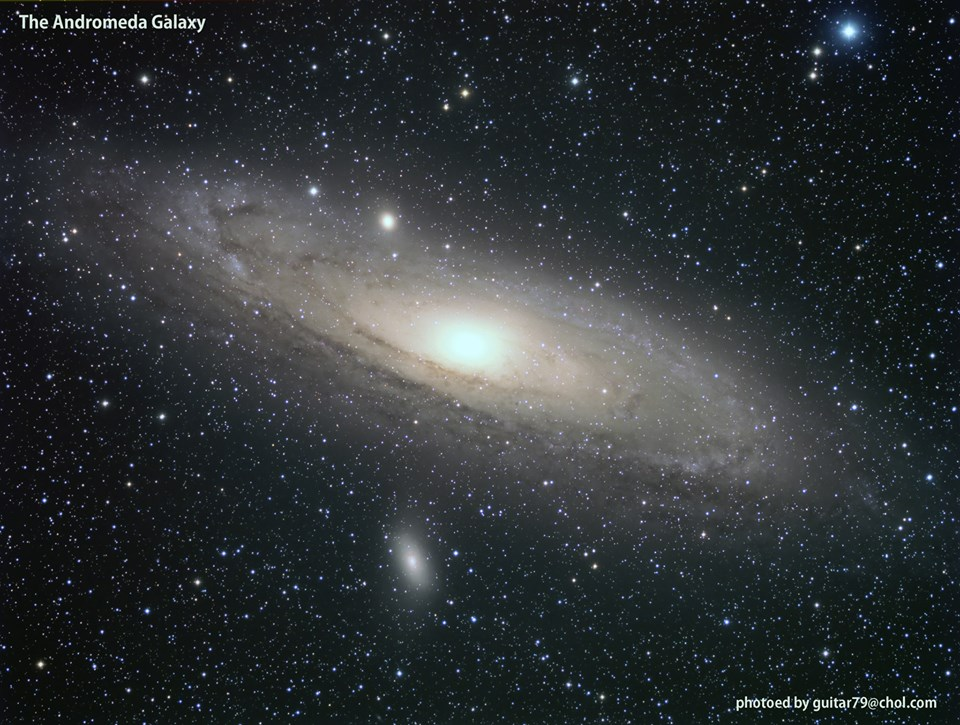
\includegraphics[width=0.8\linewidth]{Andromeda_Galaxy}
		\caption{The Andromeda galaxy : L 600s X 14 frames, RGB 400s X 6 frames each (Takahashi FSQ106-ED with 0.73X Reducer QE, Sbig ST-8300M, Takahashi EM-200 Temma 2).}
		\label{fig:The_Andromeda_Galaxy}
	\end{center}
\end{figure}

광학계에 의한 별의 상이 검출기에 정확하게 맺히도록 하기 위해서는 포커서를 정밀하게 움직여야 한다. 사진 촬영을 위한 고성능의 광학계는 포커서(Focuser)를 견고하게 만들 뿐 아니라 포커서 노브에 미동 장치가 있어 정밀하게 초점 조절이 가능하다. 하지만 포커서를 조절하기 위해 손이 포커서에 닿을 경우 그 진동이 상에 영향을 미치기 때문에 손으로 초점을 조절하는 것은 매우 어렵다. 

또한 관측을 하는 동안 온도 변화에 의해서 망원경의 초점이 변하기도 한다. 이를 해결하기 위하여 Persha (2001)는 주위 온도에 따라 변하는 초점 보정하기 위한 온도 보상 초점 방법을 연구하였다 \cite{persha2001temperature}.


\subsection{연구 목적}

본 연구에서는 천체 관측시 초점 조절 과정에서 손에 의한 진동의 영향을 받지 않고 정밀하게 포커서를 조절하기 위하여 모터를 이용하여 포커서를 돌려 초점을 조절할 수 있는 모터 포커서 컨트롤러 구동 시스템을 개발하였다. 또한 전용 ASCOM dirver를 개발하여 ASCOM을 지원하는 천문 소프트웨어를 이용하여 쉽게 사용할 수 있도록 하였다. 


\subsection{연구 문제}

%% 박기현샘 : 연구문제의 답이 결론에 제시되어야 함. 둘이 호응관계가 되도록 기술
연구 목적에 맞게 펌웨어 및 ASCOM 드라이버를 개발하기 위해서 필요한 기능들과 기술들을 생각해보았으며, 이는 다음과 같다.

1. 펌웨어에서 버튼과 디스플레이의 메뉴를 이용하여 모터를 조절할 수 있도록 한다.

2. 펌웨어에서 serialPort를 통해 버튼과 디스플레이에서 할 수 있는 기능들을 실행할 수 있도록 한다.

3. ASCOM driver이 펌웨어와 통신이 가능하도록 하고, 드라이버에서 버튼을 클릭하는 것으로 펌웨어와 같은 기능을 할 수 있도록 한다.